\chapter{TEOR\'{I}A: Fundamentos de estructura de macromol\'{e}culas} \label{macro1}


\section{Papel biol\'{o}gico de las macromol\'{e}culas: relaci\'{o}n entre secuencia, estructura y funci\'{o}n}

Los \'{a}cidos nucleicos y las prote\'\i{}nas son las dos macromol\'{e}culas biol\'{o}gicas m\'{a}s importantes.
Ambas son los canales principales de los flujos de 
informaci\'{o}n gen\'{o}mica dentro de la c\'{e}lula, que convierten en acciones moleculares el legado gen\'{e}tico
acumulado. Sabemos que el \'{a}cido desoxirribonucleico (ADN) puede guardar informaci\'{o}n gen\'{e}tica a largo 
plazo, mientras que el \'{a}cido ribonucleico (ARN) lo hace normalmente a muy corto plazo. Son las prote\'\i{}nas,
y algunas clases especiales de ARN, quienes convierten en el contexto celular esa informaci\'{o}n en acci\'{o}n. 
Para comprender c\'{o}mo realizan estas funciones es muy importante tener una idea de su estructura molecular. 
Esto debemos tenerlo siempre en cuenta en el \'{a}mbito bioinform\'{a}tico, donde a veces hablamos de genes y 
prote\'\i{}nas como entidades abstractas cuya funci\'{o}n es s\'{o}lo un verbo.


\begin{figure}
%\htmlimage{scale=1.5}
\begin{center} 
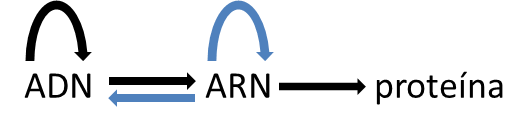
\includegraphics[width=0.8\textwidth]{flujoinfo}
\caption%[]
{
Flujos moleculares de informaci\'{o}n en la c\'{e}lula. 
Los flujos azules solamente se encuentran en algunos seres vivos, las negras son universales.
}
\label{fig:flujosinfobio}
\end{center}
\end{figure}

La funci\'{o}n biol\'{o}gica de estas mol\'{e}culas est\'{a} \'\i{}ntimamente ligada a su estructura. Por ejemplo, la estructura en doble h\'{e}lice 
del ADN es en si mismo un mecanismo de protecci\'{o}n de la informaci\'{o}n gen\'{e}tica, ya que la informaci\'{o}n est\'{a} contenida por 
duplicado, y asimismo es la base de su mecanismo de replicaci\'{o}n.


\begin{figure}
\htmlimage{scale=1.5}
\begin{center} 
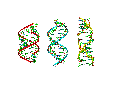
\includegraphics[width=1.0\textwidth]{dna}
\caption%[]
{
Estructura helicoidal del ADN (DNA en ingl\'{e}s) en conformaciones A, B y Z.
Figura de dominio p\'{u}blico tomada de 
\htmladdnormallink{https://en.wikipedia.org/wiki/Nucleic_acid_structure}{https://en.wikipedia.org/wiki/Nucleic_acid_structure}.
}
\label{fig:dna}
\end{center}
\end{figure}

Las macromol\'{e}culas naturales deben plegarse, es decir, deben tomar una determinada conformaci\'{o}n 
tridimensional relativamente estable para desempe\~nar su funci\'{o}n biol\'{o}gica. 
A esta conformaci\'{o}n, sostenida por una red de interacciones no covalentes, se le llama \italics{nativa} 
(ver secci\'{o}n \ref{macro1:intnocov}).
Por el contrario, las mol\'{e}culas se despliegan al perderse estas interacciones. 
Cuando una macromol\'{e}cula pierde
su estructura tridimensional nativa, normalmente pierde tambi\'{e}n su funci\'{o}n. O al menos antes lo cre\'{i}amos as\'{i}.
Ahora conocemos cada vez m\'{a}s prote\'\i{}nas intr\'\i{}nsecamente desordenadas no plegadas, 
que participan en complejos proteicos o que s\'{o}lo se pliegan al unirse a sus ligandos y reducir su entrop\'{i}a \citep{Flock2014, Riback2017}, 
que desempe\~nan funciones celulares importantes \citep{Dyson1999}. Recientemente hay mucho inter\'{e}s en estudiar estos fen\'{o}menos 
por su relaci\'{o}n con la complejidad de los organismos \citep{Yruela2017} y con prote\'{i}nas de importancia en medicina como los 
\htmladdnormallink{priones}{http://es.wikipedia.org/wiki/Prion} \citep{Sabate2015}.


\begin{figure}
\begin{center} 
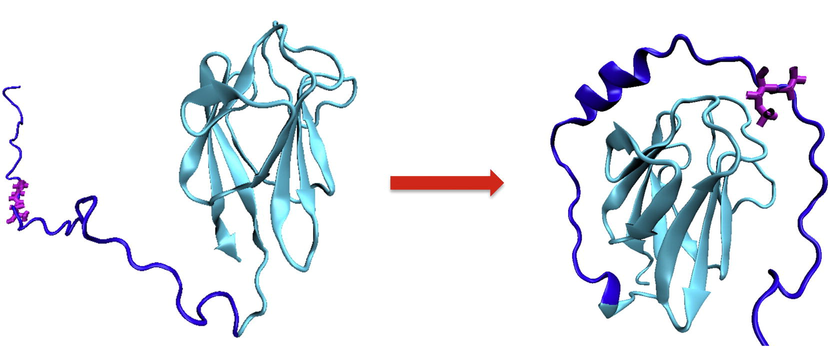
\includegraphics[width=0.7\textwidth]{disorderautoinhib}
\caption%[]
{
Algunas regiones desordenadas tienen un rol autoinhibitorio, como el fragmento en color rosa de la figura.  
Figura tomada de \cite{Trudeau2013} y reproducida con permiso de los autores.
}
\label{fig:autoinhdis}
\end{center}
\end{figure}



\section{Componentes y enlaces}

Prote\'\i{}nas y \'{a}cidos nucleicos pueden considerarse pol\'\i{}meros, mol\'{e}culas generadas por la sucesi\'{o}n de mon\'{o}meros
elegidos de un repertorio limitado. En ambos casos la secuencia de mon\'{o}meros da la especificidad biol\'{o}gica 
a cada macromol\'{e}cula. En el caso de las prote\'\i{}nas los mon\'{o}meros son amino\'{a}cidos y el repertorio
incluye \htmladdnormallink{generalmente}{http://en.wikipedia.org/wiki/Proteinogenic} 
20 distintos. Por otro lado, los \'{a}cidos nucleicos est\'{a}n compuestos por nucle\'{o}tidos (ver secci\'{o}n \ref{nts}).

\subsection{El enlace pept\'\i{}dico y los amino\'{a}cidos}
Los 20 amino\'{a}cidos que forman parte de las prote\'\i{}nas naturales est\'{a}n compuestos por un grupo amino 
y uno carboxilo unidos por el carbono \(\alpha\), del que parten diferentes cadenas laterales (R, ver 
figura \ref{fig:amino_stereo}). La cadena lateral R diferencia a los 20 amino\'{a}cidos y les confiere propiedades 
qu\'\i{}micas espec\'\i{}ficas \citep{yruela_inmaculada_2014_1067867}.

\begin{figure}
\begin{center} 
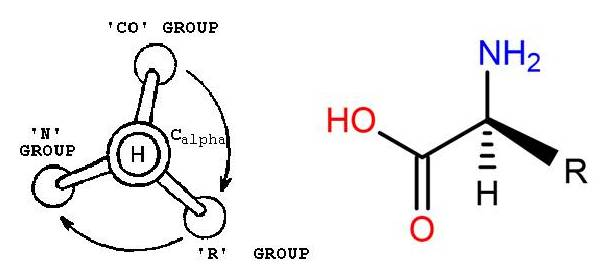
\includegraphics[]{amino_stereo}
\caption%[]
{
Estructura qu\'\i{}mica de los L-amino\'{a}cidos.
En el panel de la derecha se muestra su polaridad, con grupos con cargas positivas (en azul) y negativas (en rojo).
}
\label{fig:amino_stereo}
\end{center}
\end{figure}

\begin{figure}
\begin{center} 
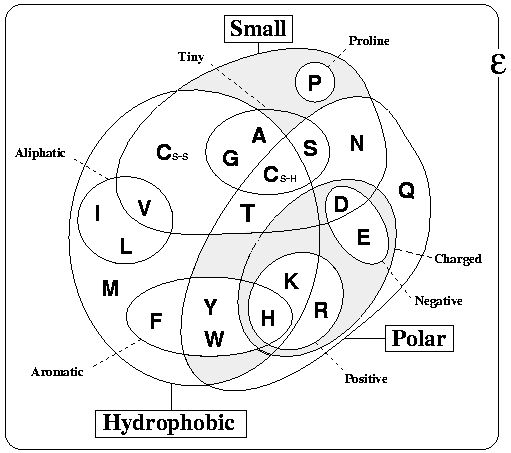
\includegraphics[width=0.3\textwidth]{amino_classif}
\caption%[]
{
Clasificaci\'{o}n de los 20 amino\'{a}cidos naturales,tomada de \htmladdnormallink{http://www.russelllab.org/aas}{http://www.russelllab.org/aas}.
La selenociste\'\i{}na, que contiene un \'{a}tomo de Se en vez de S, se considera el amino\'{a}cido 21 \citep{Santesmasses2017,Granold2018}.
}
\label{fig:amino_classif}
\end{center}
\end{figure}

\begin{figure}
\begin{center} 
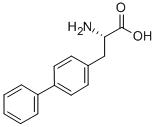
\includegraphics[]{bipA}
\caption%[]
{
L-4,4'-bifenilalanina, un amino\'{a}cido no natural empleado en biotecnolog\'{i}a.
Figura tomada de \htmladdnormallink{http://www.chemicalbook.com}{http://www.chemicalbook.com}.
}
\label{fig:bipA}
\end{center}
\end{figure}

Los amino\'{a}cidos se encadenan por medio de enlaces 
pept\'\i{}dicos para formar prote\'\i{}nas, tambi\'{e}n llamadas cadenas polipept\'\i{}dicas, como se muestra en la 
figura \ref{fig:peptide_bond}. Si excluimos las cadenas laterales R de los amino\'{a}cidos de la cadena obtenemos 
el esqueleto pept\'\i{}dico (\italics{backbone}), 
cuya geometr\'{i}a puede describirse con precisi\'{o}n conociendo los \'{a}ngulos diedros $\phi$ y $\psi$ (ver secci\'{o}n \ref{SS}).

\begin{figure}
%\htmlimage{scale=2.0}
\begin{center} 
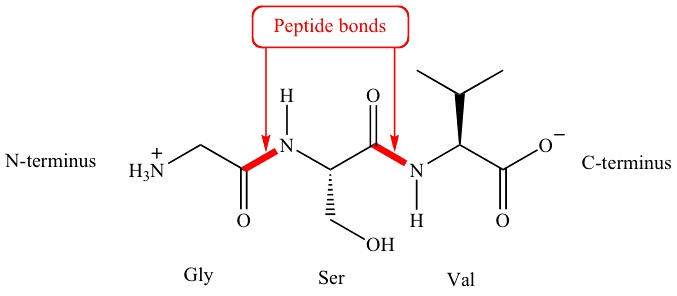
\includegraphics[width=0.8\textwidth]{peptide_bond}
\caption%[]
{
Estructura del enlace pept\'\i{}dico y la cadena polipept\'\i{}dica. Este enlace es r\'\i{}gido, plano y no permite el giro.
Figura tomada de \htmladdnormallink{http://www.chem.ucla.edu}{http://www.chem.ucla.edu}.
}
\label{fig:peptide_bond}
\end{center}
\end{figure}



\subsection{El enlace fosfodi\'{e}ster y los nucle\'{o}tidos} \label{nts}
Los nucle\'{o}tidos que forman los \'{a}cidos nucleicos se componen a su vez de mol\'{e}culas: un fosfato, una pentosa y una 
base nitrogenada. Entre el ADN y el ARN la diferencia fundamental es la pentosa que incluyen: ribosa para el ARN, 
2-desoxirribosa para el ADN. Las 4 bases nitrogenadas que pueden unirse a las pentosas dan identidad al nucle\'{o}tido.
La otra diferencia entre ADN y ARN es precisamente su repertorio de bases nitrogenadas. Comparten la adenina, la 
guanina y la citosina, mientras que la timina es espec\'\i{}fica del ADN y el uracilo del ARN.

\begin{figure}
\htmlimage{scale=1.0}
\begin{center} 
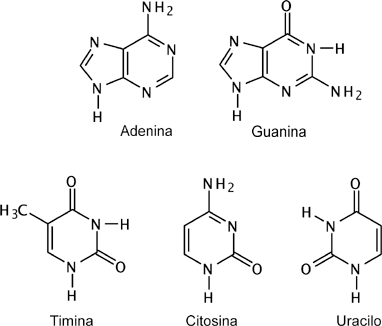
\includegraphics{basesn}
\caption%[]
{
Las 5 bases nitrogenadas de los \'{a}cidos nucleicos, tomadas de superfund.pharmacy.arizona.edu.
A y G son purinas, mientras que C, T y U son pirimidinas.
}
\label{fig:basesn}
\end{center}
\end{figure}

\begin{figure}
\htmlimage{scale=1.0}
\begin{center} 
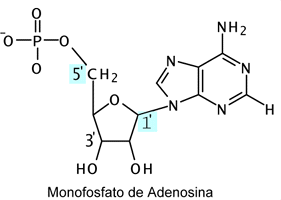
\includegraphics{nucleotido}
\caption%[]
{
Ejemplo de nucle\'{o}tido, tomado de superfund.pharmacy.arizona.edu.
}
\label{fig:nucleotido}
\end{center}
\end{figure}

\begin{figure}
%\htmlimage{scale=1.0}
\begin{center} 
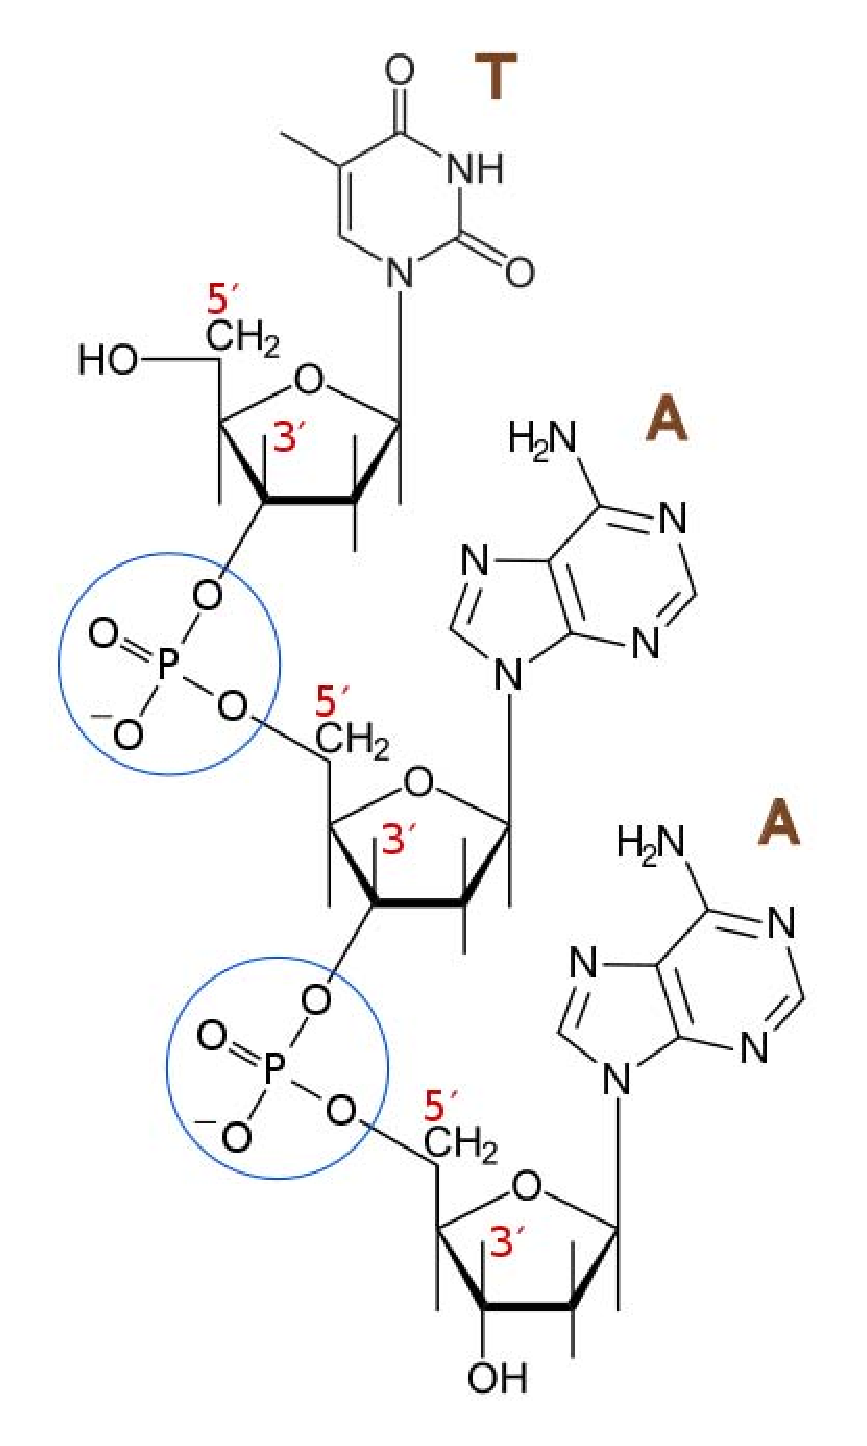
\includegraphics{fosfodiester}
\caption%[]
{
Dibujo de un trinucle\'{o}tido 5'-TAA-3' mostrando dos enlaces fosfodi\'{e}ster consecutivos, 
tomado de \htmladdnormallink{http://www.wikiwand.com}{http://www.wikiwand.com/gl/Enlace_fosfodi\%C3\%A9ster}.
Figura reproducida con permiso de los autores.
}
\label{fig:fosfodiester}
\end{center}
\end{figure}

Los nucle\'{o}tidos se enlazan por medio de enlaces fosfodi\'{e}ster %(ver figura \ref{fig:fosfodiester}) 
para formar polinucle\'{o}tidos, es decir, cadenas de ADN o ARN, cuyo sentido viene definido por los 2 carbonos que intervienen en
este enlace. 

\subsection{Interacciones no covalentes en las macromol\'{e}culas} \label{macro1:intnocov}

Adem\'{a}s de los enlaces pept\'\i{}dico y fosfodi\'{e}ster, debemos conocer otras interacciones at\'{o}micas no covalentes 
m\'{a}s d\'{e}biles, pero muy importantes para comprender las macromol\'{e}culas \citep{Lehninger1982}. Son sobre todo de estos tipos: 

\begin{itemize}
\item Interacciones hidrof\'{o}bicas entre solutos en soluciones acuosas. 
Se consideran hidrof\'{o}bicas aquellas sustancias que son repelidas por el agua o que no se pueden mezclar con ella.

\item \htmladdnormallink{Atracci\'{o}n de van der Waals}{http://es.wikipedia.org/wiki/Fuerzas\_de\_van\_der\_Waals} 
entre \'{a}tomos no cargados, hasta el punto en que casi se solapan sus orbitales externos.

\item \htmladdnormallink{Interacciones electrost\'{a}ticas}{http://es.wikipedia.org/wiki/Electrost\%C3\%A1tica}
inversamente proporcionales a la distancia entre \'{a}tomos de cargas propias o inducidas. Dentro de las prote\'{i}nas
reciben a veces el nombre de 
\htmladdnormallink{puentes salinos}{http://es.wikipedia.org/wiki/Estructura\_de\_las\_prote\%C3\%ADnas\#Interacciones\_carga\-carga},
y son m\'{a}s frecuentes entre residuos cercanos en secuencia \citep{Donald2011}.

\item \htmladdnormallink{Puentes de H}{http://es.wikipedia.org/wiki/Enlace\_por\_puente\_de\_hidr\%C3\%B3geno}, 
de longitud fija, entre \'{a}tomos de cargas opuestas que son adem\'{a}s parte de enlaces 
covalentes parciales. En prote\'\i{}nas es com\'{u}n entre grupos -NH y O=C-, puesto que en estos casos el H tiene 
carga parcial positiva y el O negativa. En los \'{a}cidos nucleicos encontramos sobre todo los puentes que sostienen los 
\htmladdnormallink{pares de bases}{http://en.wikipedia.org/wiki/Base\_pair}.

\end{itemize}


\section{An\'{a}lisis jer\'{a}rquico de la estructura de macromol\'{e}culas}

La estructura de \'{a}cidos nucleicos y prote\'\i{}nas puede analizarse de forma jer\'{a}rquica en 4 niveles, partiendo de
la estructura primaria, su secuencia de mon\'{o}meros, hasta llegar a su estructura cuaternaria, el nivel de asociaci\'{o}n
de diferentes cadenas. 

\subsection{Estructura primaria} 

La estructura primaria de una prote\'\i{}na se corresponde con la secuencia lineal de amino\'{a}cidos codificada
en su correspondiente unidad de transcripci\'{o}n y suele representarse por medio de una cadena donde cada 
letra identifica a un amino\'{a}cido o residuo. Por ejemplo, los primeros 30 amino\'{a}cidos de la prote\'\i{}na 
insulina de la mosca \italics{Drosophila melanogaster} son:\\ 

\texttt{MFSQHNGAAV HGLRLQSLLI AAMLTAAMAM...}\\

donde por ejemplo M es metionina, Q es glutamina o A es alanina. % (ver tabla \ref{tab:amino}). 
El sentido de la cadena es desde el extremo amino-terminal hacia el carboxilo-terminal. 

\begin{table}[h]
\begin{center}
\begin{scriptsize}
\begin{tabular}{|l|l|l|l|l|l|l|}\hline
A & ALA & Alanina & & M & MET & Metionina\\   
C & CYS & Ciste\'\i{}na & & N & ASN & Asparagina\\
D & ASP & Aspartato & & P & PRO & Prolina\\ 
E & GLU & Glutamato & & Q & GLN & Glutamina\\  
F & PHE & Fenilalanina & & R & ARG & Arginina\\
G & GLY & Glicina & & S & SER & Serina\\      
H & HIS & Histidina & & T & THR & Treonina\\    
I & ILE & Isoleucina & & V & VAL & Valina\\   
K & LYS & Lisina & & W & TRP & Tript\'{o}fano\\
L & LEU & Leucina & & Y & TYR & Tirosina\\
X & -   & desconocido & & & &\\\hline
\end{tabular}
\end{scriptsize}
\end{center}
\caption%[]
{Nomenclatura de los 20 amino\'{a}cidos esenciales}
\label{tab:amino}
\end{table}

De igual manera, la estructura primaria de los \'{a}cidos nucleicos es su secuencia de nucle\'{o}tidos, que tiene un sentido
dado por la direcci\'{o}n de los enlaces fosfodi\'{e}ster. De igual modo se suele representar de forma simplificada, asignando
una sola letra a cada nucle\'{o}tido, o mejor dicho, a cada base nitrogenada. Adem\'{a}s se suele usar el sentido 5'-3'.
Por ejemplo, el principio del gen de la insulina de la mosca \italics{Drosophila melanogaster} tiene una secuencia similar a:\\

\texttt{5' atgtttagcc agcacaacgg tgcagcagta 3'}\\

donde A es adenina, T timina, C citosina y G guanina. En el caso del ADN, que como veremos suele formar una doble h\'{e}lice
antiparalela, se sobreentiende que hay una secuencia complementaria que corre en sentido opuesto. En este caso ser\'\i{}a:\\

\texttt{5' atgtttagcc agcacaacgg tgcagcagta 3'}\\
\texttt{3' tacaaatcgg tcgtgttgcc acgtcgtcat 5'}\\

En el caso de secuencias codificantes, la secuencia primaria se puede representar en forma de codones o tr\'{i}os de pares de bases, donde
cada uno codifica para un amino\'{a}cido o un cod\'{o}n STOP:\\

\texttt{5' atg ttt agc cag cac aac ggt gca tga 3'}\\
\texttt{3' tac aaa tcg gtc gtg ttg cca cgt act 5'}\\

La estructura primaria en nucle\'{o}tidos es por tanto el soporte f\'{i}sico de las secuencias codificantes que son posteriormente 
traducidas a prote\'\i{}nas. Por tanto, si ocurren mutaciones en un gen es posible que la secuencia codificante correspondiente se vea alterada. 
Se pueden dar varios tipos de mutaciones, tanto si son sustituciones de un nucle\'{o}tido (SNP), inserciones o deleciones:

\begin{itemize}
\item Sustituciones sin\'{o}nimas que cambian un cod\'{o}n pero no el amino\'{a}cido correspondiente.
\item Sustituciones no sin\'{o}nimas que cambian un cod\'{o}n y el amino\'{a}cido correspondiente. En la literatura se llaman mutaciones \italics{missense}.
\item Sustituciones, inserciones o deleciones que introducen un cod\'{o}n STOP prematuro. En la literatura se llaman mutaciones \italics{nonsense}.
\item Inserciones o deleciones que alteran el marco de lectura, o los bordes entre exones e intrones, y por tanto el p\'{e}ptido resultante.
\end{itemize}


\subsection{Estructura secundaria} \label{SS}

Para neutralizar las cargas polares del esqueleto pept\'\i{}dico, las prote\'\i{}nas adoptan conformaciones
que maximizan la formaci\'{o}n de puentes de hidr\'{o}geno, gracias a la libertad de giro de los enlaces situados 
inmediatamente antes y despu\'{e}s del enlace pept\'\i{}dico. Esto lo hacen principalmente formando \(\alpha\)-h\'{e}lices 
dextr\'{o}giras, l\'{a}minas \(\beta\), como se muestra en las figuras \ref{fig:est2protH}, \ref{fig:est2protH2}, \ref{fig:est2protE} y 
\ref{fig:est2protE2}, y  giros de varios tipos, en menor medida.

\begin{figure}
%\htmlimage{scale=2.0}
\begin{center} 
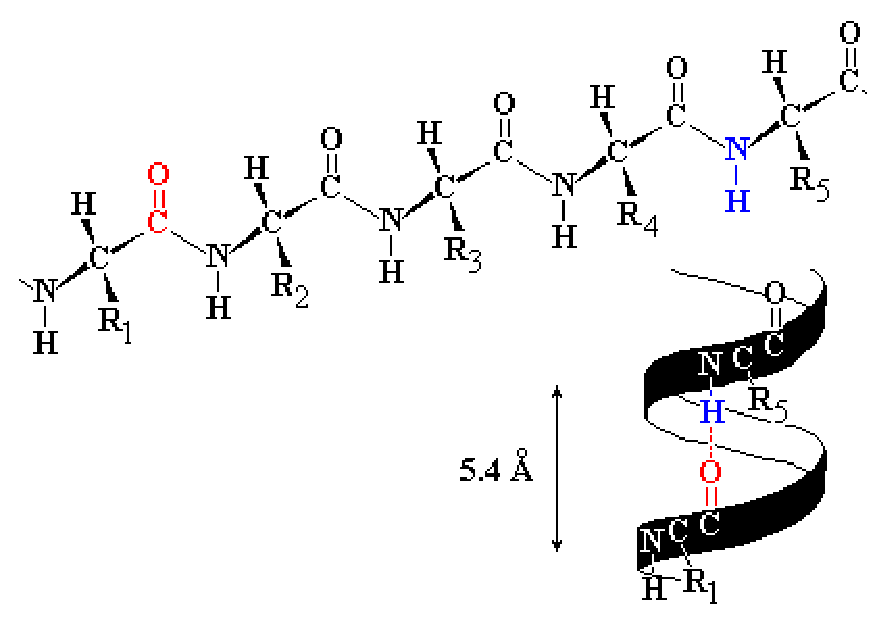
\includegraphics[width=0.8\textwidth]{est2protH}
\caption%[]
{
Esquema de $\alpha$-h\'{e}lice en una cadena polipept\'\i{}dica,
tomado de \htmladdnormallink{http://www.chembio.uoguelph.ca}{http://www.chembio.uoguelph.ca}.
}
\label{fig:est2protH}
\end{center}
\end{figure}

\begin{figure}
\begin{center} 
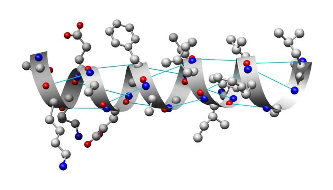
\includegraphics{est2protH2}
\caption%[]
{
$\alpha$-h\'{e}lice mostrando cadenas laterales y puentes de hidr\'{o}geno entre residuos vecinos (en azul),
tomada de \htmladdnormallink{http://structuralbioinformatics.com}{http://structuralbioinformatics.com}.
}
\label{fig:est2protH2}
\end{center}
\end{figure}

\begin{figure}
\htmlimage{scale=1.0}
\begin{center} 
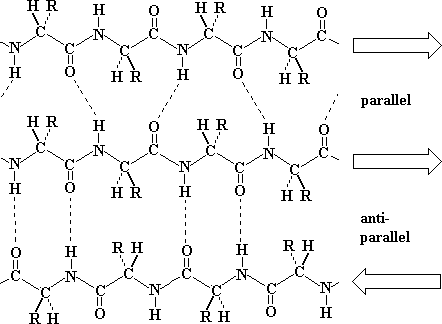
\includegraphics{est2protE}
\caption%[]
{
Esquema de las dos disposiciones posibles (paralelas y anti-paralelas) de l\'{a}minas beta en cadenas polipept\'\i{}dicas,
tomado de \htmladdnormallink{http://www.chembio.uoguelph.ca}{http://www.chembio.uoguelph.ca}.
}
\label{fig:est2protE}
\end{center}
\end{figure}

\begin{figure}
%\htmlimage{scale=1.0}
\begin{center} 
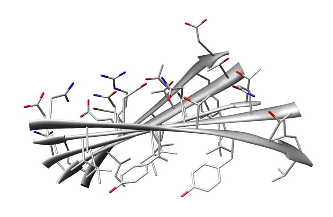
\includegraphics{est2protE2}
\caption%[]
{
Diagrama de l\'{a}minas beta antiparalelas mostrando la orientaci\'{o}n a ambos lados del plano de las cadenas laterales,
tomado de \htmladdnormallink{http://structuralbioinformatics.com}{http://structuralbioinformatics.com}.
}
\label{fig:est2protE2}
\end{center}
\end{figure}

La estructura secundaria de las prote\'{i}nas se puede codificar
de manera similar a la secuencia primaria, asignando a cada residuo una letra que identifica el estado de estructura secundaria en que se encuentra. 
Se suele identificar a los residuos de una $\alpha$-h\'{e}lice con H, los de una l\'{a}mina \(\beta\) con E y los dem\'{a}s 
con C, del ingl\'{e}s \italics{coil}. \'{E}sta ser\'{i}a la clasificaci\'{o}n simple de 3 estados,
que puede afinarse m\'{a}s llegando a \htmladdnormallink{8 estados}{https://en.wikipedia.org/wiki/Protein_secondary_structure#DSSP_H-bond_definition}:

\begin{table}[h]
\begin{center}
\begin{scriptsize}
\begin{tabular}{|l|l|}\hline
G & h\'{e}lice $3_{10}$ con vuelta de 3 residuos\\   
H & $\alpha$-h\'{e}lice con vuelta de 4 residuos\\
I & $\pi$-h\'{e}lice con vuelta de 5 residuos\\ 
T & giros de 3-5 residuos con puentes de H entre residuos vecinos\\  
E & conformaci\'{o}n extendida de l\'{a}mina \(\beta\)\\
B & puente $\beta$ entre segmentos de tres residuos en conformaci\'{o}n extendida $\beta$\\      
S & giro de gran curvatura sin puentes de H\\    
C & resto de conformaciones\\   
\end{tabular}
\end{scriptsize}
\end{center}
\caption%[]
{
Estados de estructura secundaria definidos por el algoritmo DSSP en base a patrones de puentes de hidr\'{o}geno.
}
\label{tab:SS8}
\end{table} 
%los giros soportados por puesntes de T (del ingl\'{e}s \italics{turn}) o B (de horquilla $\beta$, \italics {hairpin}). 

La misma secuencia que vimos antes podr\'{i}a tener esta estructura secundaria de 3 estados:

\texttt{MFSQHNGAAV HGLRLQSLLI AAMLTAAMAM...}\\
\texttt{EEEECCEEEE HHHHHHHHHH CCCCCCCCCC...}\\

Cuando forman parte de un elemento de estructura secundaria,
los amino\'{a}cidos adoptan conformaciones caracter\'{i}sticas, que se pueden resumir en forma de 
\htmladdnormallink{diagramas de Ramachandran}{http://en.wikipedia.org/wiki/Ramachandran_plot} \citep{Ramachandran1968}, 
que muestran la distribuci\'{o}n de valores de los \'{a}ngulos $\phi$ y $\psi$ observados a la largo del esqueleto de una prote\'{i}na:

\begin{figure}
\begin{center} 
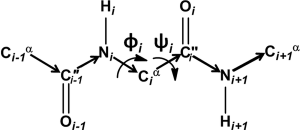
\includegraphics[width=0.8\textwidth]{phipsi3}
\caption%[fi y psi en el esqueleto pept?dico]
{
\'{A}ngulos diedros en el esqueleto proteico, figura tomada de \citep{Balaji2017}.
}
\label{fig:psiphi}
\end{center}
\end{figure}
%http://employees.csbsju.edu/HJAKUBOWSKI

\begin{figure}
\begin{center} 
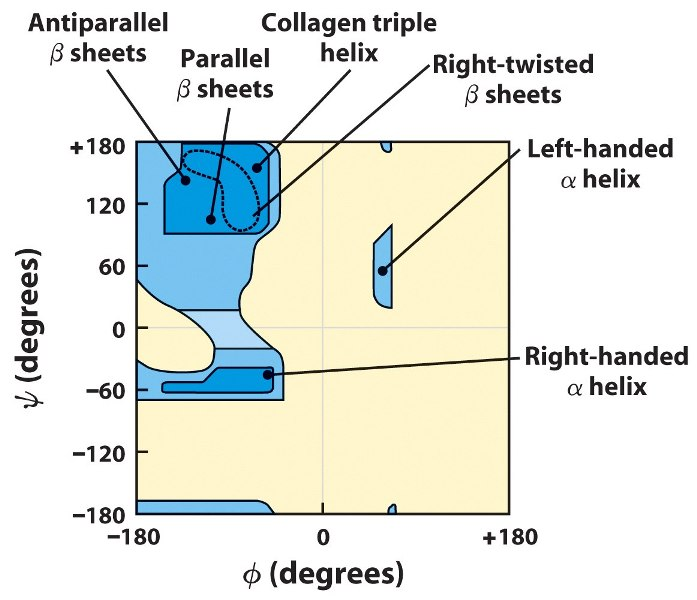
\includegraphics{ramachandranWiki}
\caption
{
Diagrama de Ramachandran tomado de \htmladdnormallink{wikimedia}{https://commons.wikimedia.org/wiki/File:Ramachandran\%27s_Diagram.jpg}.
Figura reproducida con permiso de sus autores.
}
\label{fig:ramachandran}
\end{center}
\end{figure}

%%%%%%%%%%%%%%%%%%%%%%%%%%%%%%%%%%%%%%%%%%%%

La estructura secundaria de los \'{a}cidos nucleicos est\'{a} tambi\'{e}n basada en la formaci\'{o}n de puentes de 
hidr\'{o}geno, dada la naturaleza polar de los nucle\'{o}tidos. Para el caso del ADN, como se muestra 
en la figura \ref{fig:est2adn}, el repertorio de puentes de hidr\'{o}geno posibles es muy limitado: 
adenina (A) con timina (T) y guanina (G) con citosina (C).

\begin{figure}
\htmlimage{scale=1.0}
\begin{center} 
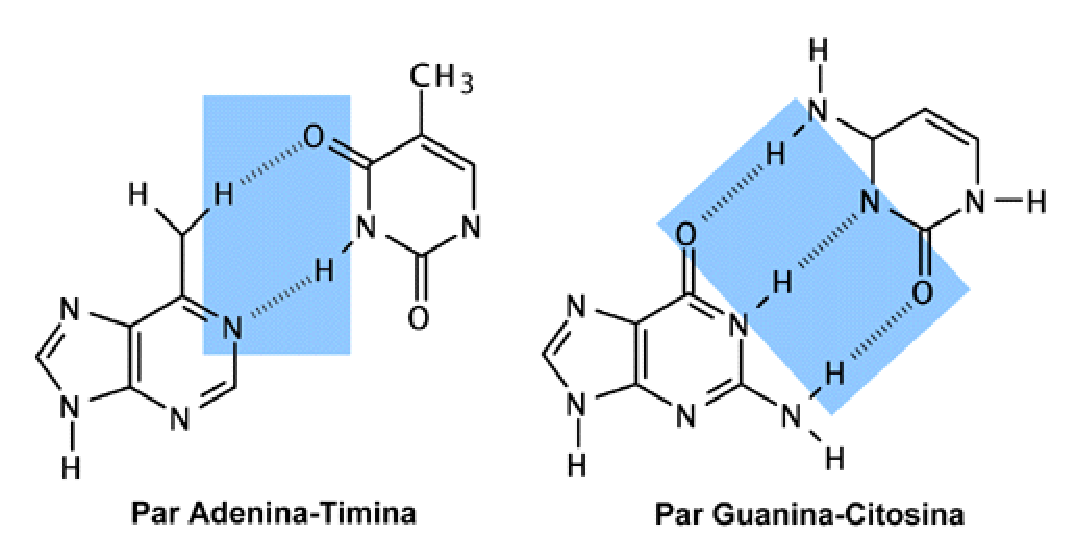
\includegraphics{est2adn}
\caption%[]
{
Posibles emparejamientos de bases en el ADN, 
figura tomada de superfund.pharmacy.arizona.edu.
}
\label{fig:est2adn}
\end{center}
\end{figure}

Estos emparejamientos son la base de la estructura secundaria de los \'{a}cidos nucleicos, que suelen ser 
patrones repetidos helicoidales. En el caso del ADN se suelen formar entre dos polinucle\'{o}tidos de secuencia 
complementaria, mientras que en el ARN son estructuras (\italics{stems},\italics{loops},...) 
que se forman dentro del mismo polinucle\'{o}tido, como se muestra en la siguiente figura:

\begin{figure}
%\htmlimage{scale=2.0}
\begin{center} 
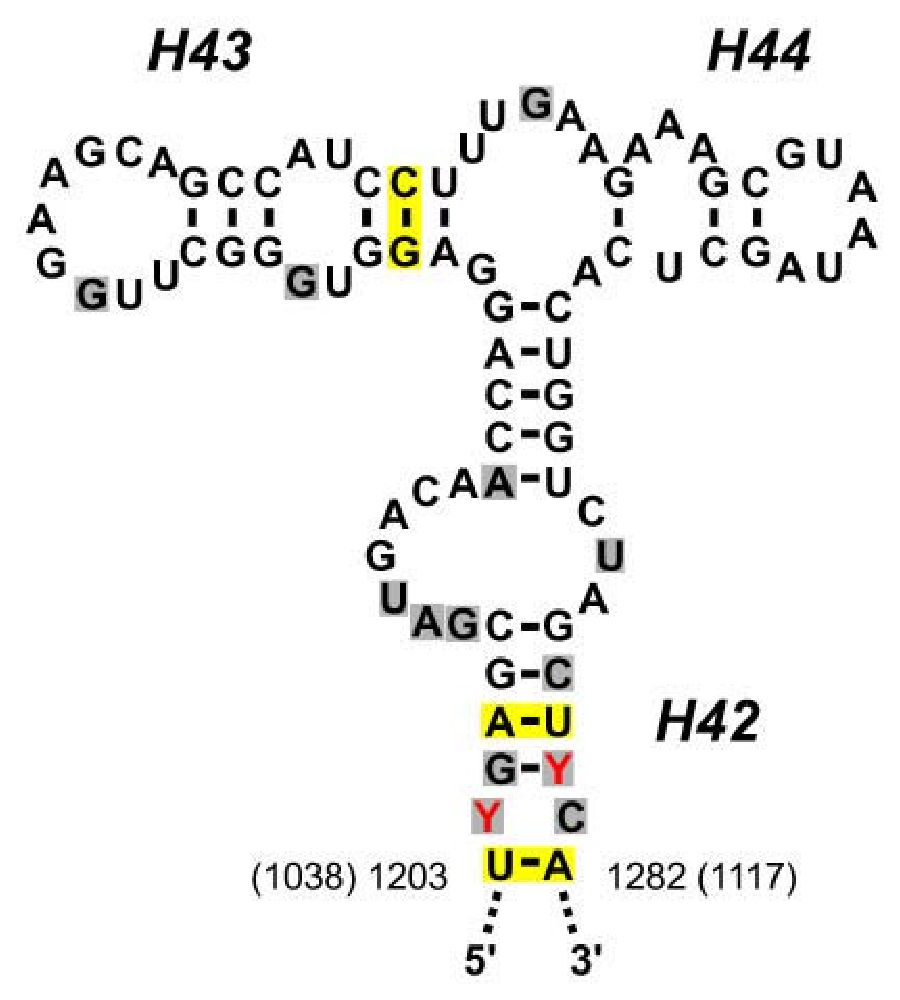
\includegraphics[width=0.8\textwidth]{est2arn}
\caption%[]
{
Ejemplo de estructura secundaria de una mol\'{e}cula de ARN mostrando la formaci\'{o}n de tallos entre segmentos alejados en secuencia.
La secuencia es la del consenso del rRNA 26S mitocondrial de Marchantia, Physcomitrella y otras plantas. 
Las posiciones coloreadas cambian en algunas especies, como se describe en \cite{Mower2009}.
Figura reproducida con permiso de los autores.
}
\label{fig:est2arn}
\end{center}
\end{figure}
%https://openi.nlm.nih.gov/detailedresult.php?img=PMC2780418_1471-2148-9-265-3&req=4

\subsection{Estructura terciaria y cuaternaria} \label{estr34}

La mayor\'\i{}a de las prote\'\i{}nas forman gl\'{o}bulos compactos al plegarse, compuestos de 
elementos de estructura secundaria organizados de una forma espec\'\i{}fica y unidos por lazos (\italics{loops} en ingl\'{e}s).
% JFR
%"...compuestos de elementos de estructura secundaria organizados de una forma espec?fica y unidos por lazos (loops en ingl?s).", 
%para distinguir de conformaciones como molten globule, por ej., que est?n formados por elementos de estructura secundaria pero 
%sin una organizaci?n espec?fica.
Las unidades globulares de plegamiento pueden llamarse 
\htmladdnormallink{dominios}{http://kinemage.biochem.duke.edu/teaching/anatax/html/anatax.2i.html} \citep{Porter2012}, 
y tienen en su interior sobre todo cadenas laterales hidrof\'{o}bicas \citep{Isom2010}, 
mostrando hacia el solvente los lazos \citep{Branden1999}. 
En raras ocasiones, una prote\'\i{}na puede formar nudos al plegarse \citep{Potestio2010,King2010} o 
agregarse como amiloides \citep{Schnabel2010}. 
Aunque no es una definici\'{o}n universal, en general un dominio tiene autonom\'{i}a funcional y termodin\'{a}mica y una historia evolutiva.
Desde el punto de vista de la secuencia primaria, un dominio puede representarse por las secuencias alineadas de las
prote\'\i{}nas que lo contienen.


Las clasificaciones estructurales de prote\'\i{}nas se hacen generalmente a nivel de dominios, como en el caso de
\htmladdnormallink{SCOP}{http://scop.berkeley.edu}, \htmladdnormallink{CATH}{http://www.cathdb.info} o
la \htmladdnormallink{taxonom\'\i{}a de Richardson}{http://kinemage.biochem.duke.edu/teaching/anatax},
aunque tambi\'{e}n se han propuesto otros esquemas, como la tabla peri\'{o}dica de \cite{Taylor2002}, donde 
la unidad b\'{a}sica de plegamiento es una combinaci\'{o}n compacta de elementos de estructura secundaria 
sostenida por una red de contactos que coevoluciona \citep{Mackenzie2017,Granata2017}. 
Se puede ampliar este tema en \citet{pascual_garcia_alberto_2014_1066350}.

\begin{figure}
\begin{center} 
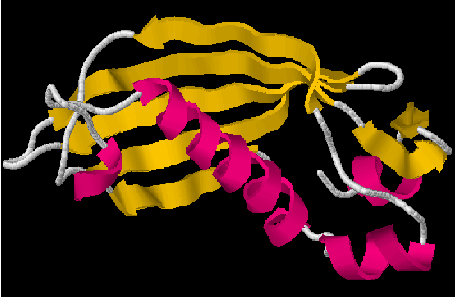
\includegraphics{1bvq}
\caption%[]
{
Estructura terciaria de una prote\'\i{}na (tioesterasa), con los elementos de
estructura secundaria coloreados (amarillo para la l\'{a}minas betas, rosa para alfa-h\'{e}lices y blanco para los lazos). 
Figura exportada con el programa \htmladdnormallink{RasMol}{http://rasmol.org/}.
}
\label{fig:1bvq}
\end{center}
\end{figure}

\begin{figure}
\begin{center} 
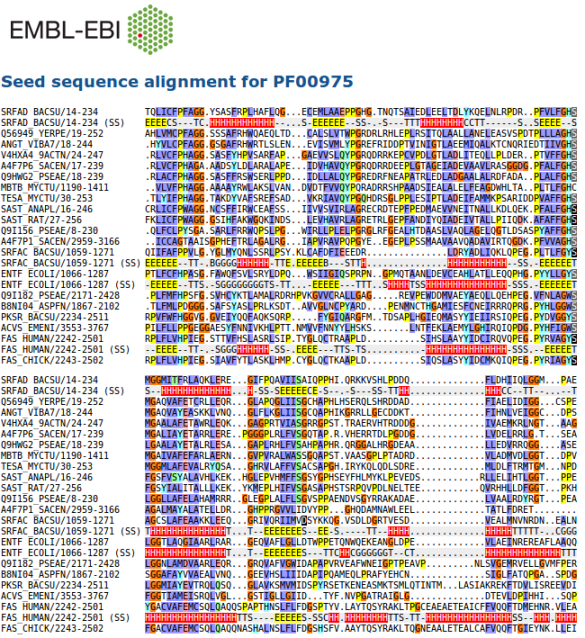
\includegraphics{thiosterase}
\caption%[]
{
Alineamiento de secuencias primarias y secundarias de diferentes dominios de tipo tioesterasa
anotados en la base de datos \htmladdnormallink{Pfam}{https://pfam.xfam.org/family/Thioesterase}.
Se colorean con distintos colores las columnas con G, P, las cadenas laterales peque\~{n}as o hidrof\'{o}bicas 
(C,A,V,L,I,M,F,W), residuos con grupo hidroxilo o amina (S,T,N,Q), los cargados (D,E,R,K)
y finalmente los residuos H o Y.
}
\label{fig:1bvq}
\end{center}
\end{figure}


\begin{figure}
\begin{center} 
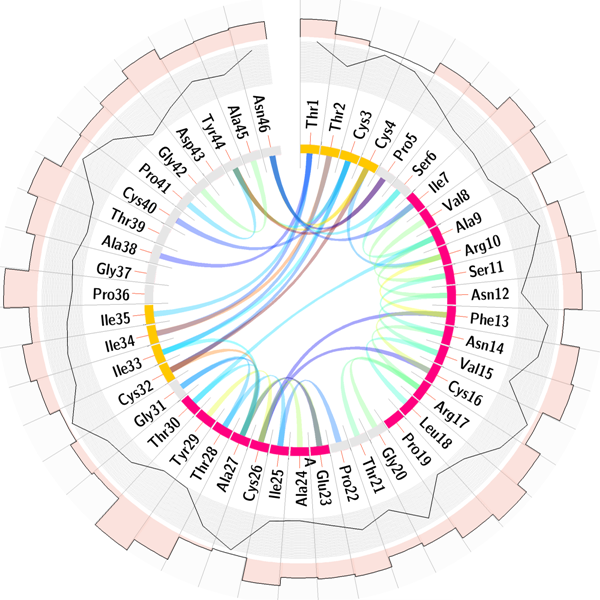
\includegraphics{1crn}
\caption%[]
{
Representaci\'{o}n estilo \htmladdnormallink{CIRCOS}{http://circos.ca} de la 
estructura terciaria de una prote\'\i{}na, con los elementos de estructura secundaria coloreados. 
Figura creada con el programa \htmladdnormallink{PDBCirclePlot}{http://sacan.biomed.drexel.edu/pdbcircleplot}.
}
\label{fig:1crn}
\end{center}
\end{figure}

Otra manera de representar la estructura terciaria es por medio de matrices de contactos, 
que resumen en forma matricial los contactos observados entre los residuos de una secuencia. 
Es habitual que las matrices de contactos o \italics{contact maps}
se calculen excluyendo los contactos entre residuos inmediatamente vecinos.
La siguiente figura muestra de qu\'{e} manera se reflejan los elementos de estructura
secundaria en una matriz de contactos, donde los ejes son los residuos ordenados por su posici\'{o}n en la secuencia.

\begin{figure}
\begin{center} 
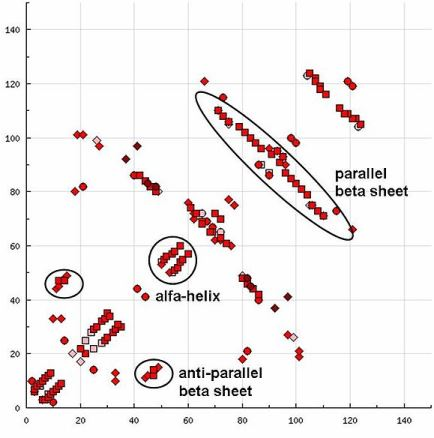
\includegraphics{SScontactMap}
\caption%[]
{
Elementos de estructura secundaria en una matriz de contactos.
Figura reproducida con permiso de 
\htmladdnormallink{http://en.wikipedia.org/wiki/Protein_contact_map}{http://en.wikipedia.org/wiki/Protein_contact_map}.
}
\label{fig:SScontacts}
\end{center}
\end{figure}

Esta manera de condensar una estructura terciaria es literalmente el fundamento de la resoluci\'{o}n de estructuras por NMR 
(ver secci\'{o}n \ref{metodosExp}), donde las observaciones experimentales de partida son esencialmente contactos at\'{o}micos 
entre residuos. 

\begin{figure}
\begin{center} 
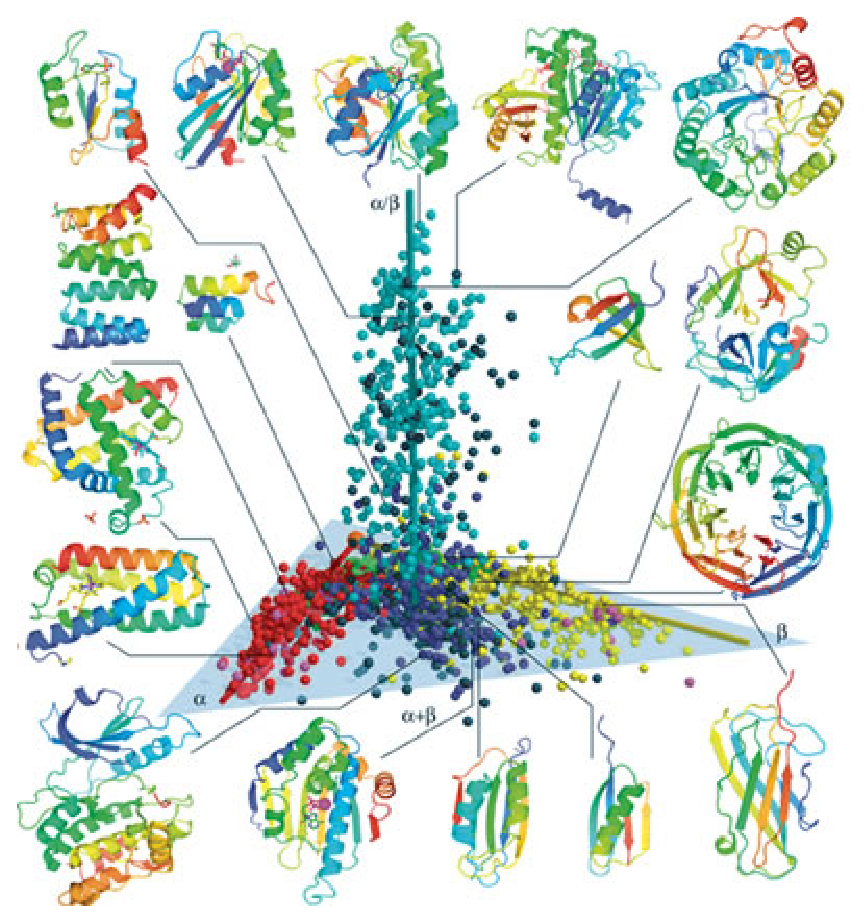
\includegraphics{foldclassification}
\caption%[]
{
Distribuci\'{o}n de plegamientos de prote\'\i{}nas de las 4 clases principales de 
\htmladdnormallink{SCOP}{http://scop.berkeley.edu} ($\alpha$, $\beta$, $\alpha+\beta$, $\alpha/\beta$)
tras reducir la dimensionalidad de los datos originales por escalado multidimensional.
Figura tomada de \cite{Hou2005}. Copyright (2005) National Academy of Sciences.
}
\label{fig:foldclassif}
\end{center}
\end{figure}

% no es gratuito su uso en clase
%\begin{figure}
%\begin{center} 
%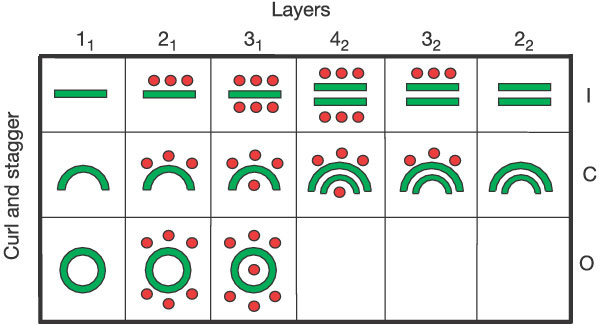
\includegraphics{fold_periodic_table}
%\caption%[]
%{
%Tabla peri\'{o}dica de topolog\'{i}as de dominios globulares, tomada de \cite{Taylor2002}.
%}
%\label{fig:foldtable}
%\end{center}
%\end{figure}

\begin{figure}
\begin{center} 
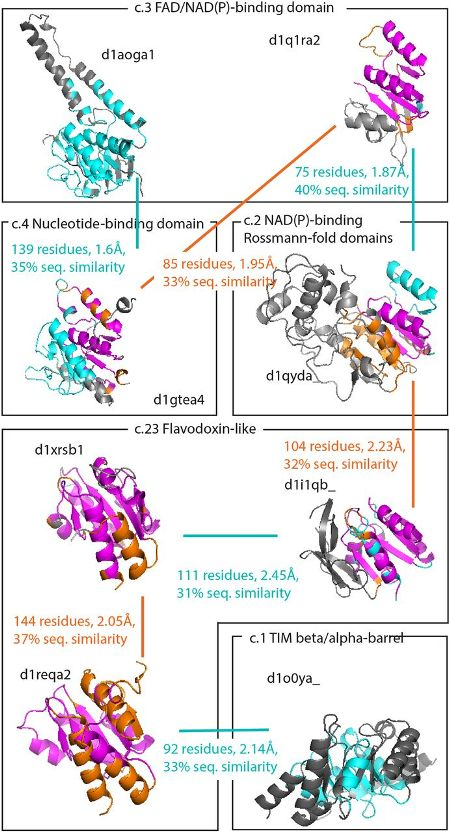
\includegraphics{domain_walk}
\caption%[]
{
Posible camino evolutivo que conecta 5 plegamientos distintos de la clase $\alpha/\beta$ de SCOP.
La ruta visita 8 dominios distintos que comparten parte de su topolog\'{i}a y estructura.
Para cada pareja de dominios se indica el total de residuos alineados, el RMSD y el \% similitud de secuencia.
Figura tomada de \cite{Nepomnyachiy2014} con permiso de los autores.
}
\label{fig:foldpaths}
\end{center}
\end{figure}
%http://www.pnas.org/page/about/rights-permissions


En cuanto a los \'{a}cidos nucleicos, su estructura terciaria es muy distinta seg\'{u}n se trate de ADN o ARN.\\

El ADN suele formar una doble h\'{e}lice dextr\'{o}gira antiparalela donde dos cadenas polinucleot\'\i{}dicas, de secuencia complementaria,
corren en sentidos opuestos, como se muestra en la figura \ref{fig:dna3}. El grado de enrollamiento 
del ADN puede variar e incluso sabemos que hay al menos 
\htmladdnormallink{3 tipos}{http://en.wikipedia.org/wiki/DNA_structure#DNA_helix_geometries}
de dobles h\'{e}lices posibles, una de ellas lev\'{o}gira, y una triple h\'{e}lice.

%\begin{figure}
%\htmlimage{scale=1.5}
%\begin{center} 
%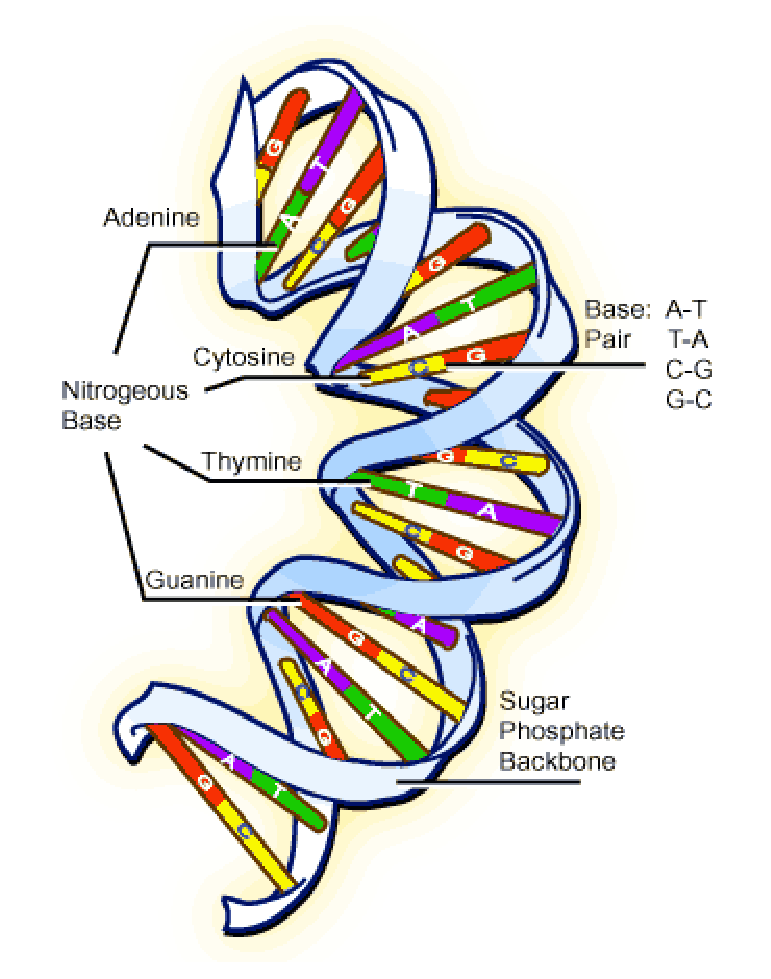
\includegraphics[width=0.8\textwidth]{dna2}
%\caption%[]
%{
%Esquema de la doble h\'{e}lice antiparalela del ADN, tomada de
%\htmladdnormallink{http://www.bioteach.ubc.ca}{http://www.bioteach.ubc.ca}.
%}
%\label{fig:dna2}
%\end{center}
%\end{figure}

\begin{figure}
\begin{center} 
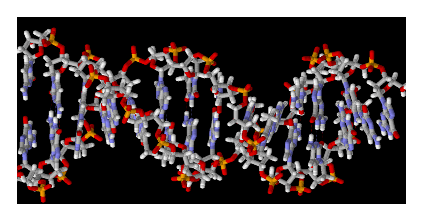
\includegraphics{dna3}
\caption%[]
{
Estructura at\'{o}mica en doble h\'{e}lice antiparalela del ADN, generada con \htmladdnormallink{RasMol}{http://rasmol.org/}. 
}
\label{fig:dna3}
\end{center}
\end{figure}

%El ARN, por otro lado, puede formar estructuras terciarias tan complejas como las de las prote\'\i{}nas. En la figura 
%\ref{fig:rna} se muestra el ARN de transferencia de levadura para la fenilalanina.
%
%\begin{figure}
%\htmlimage{scale=1.0}
%\begin{center} 
%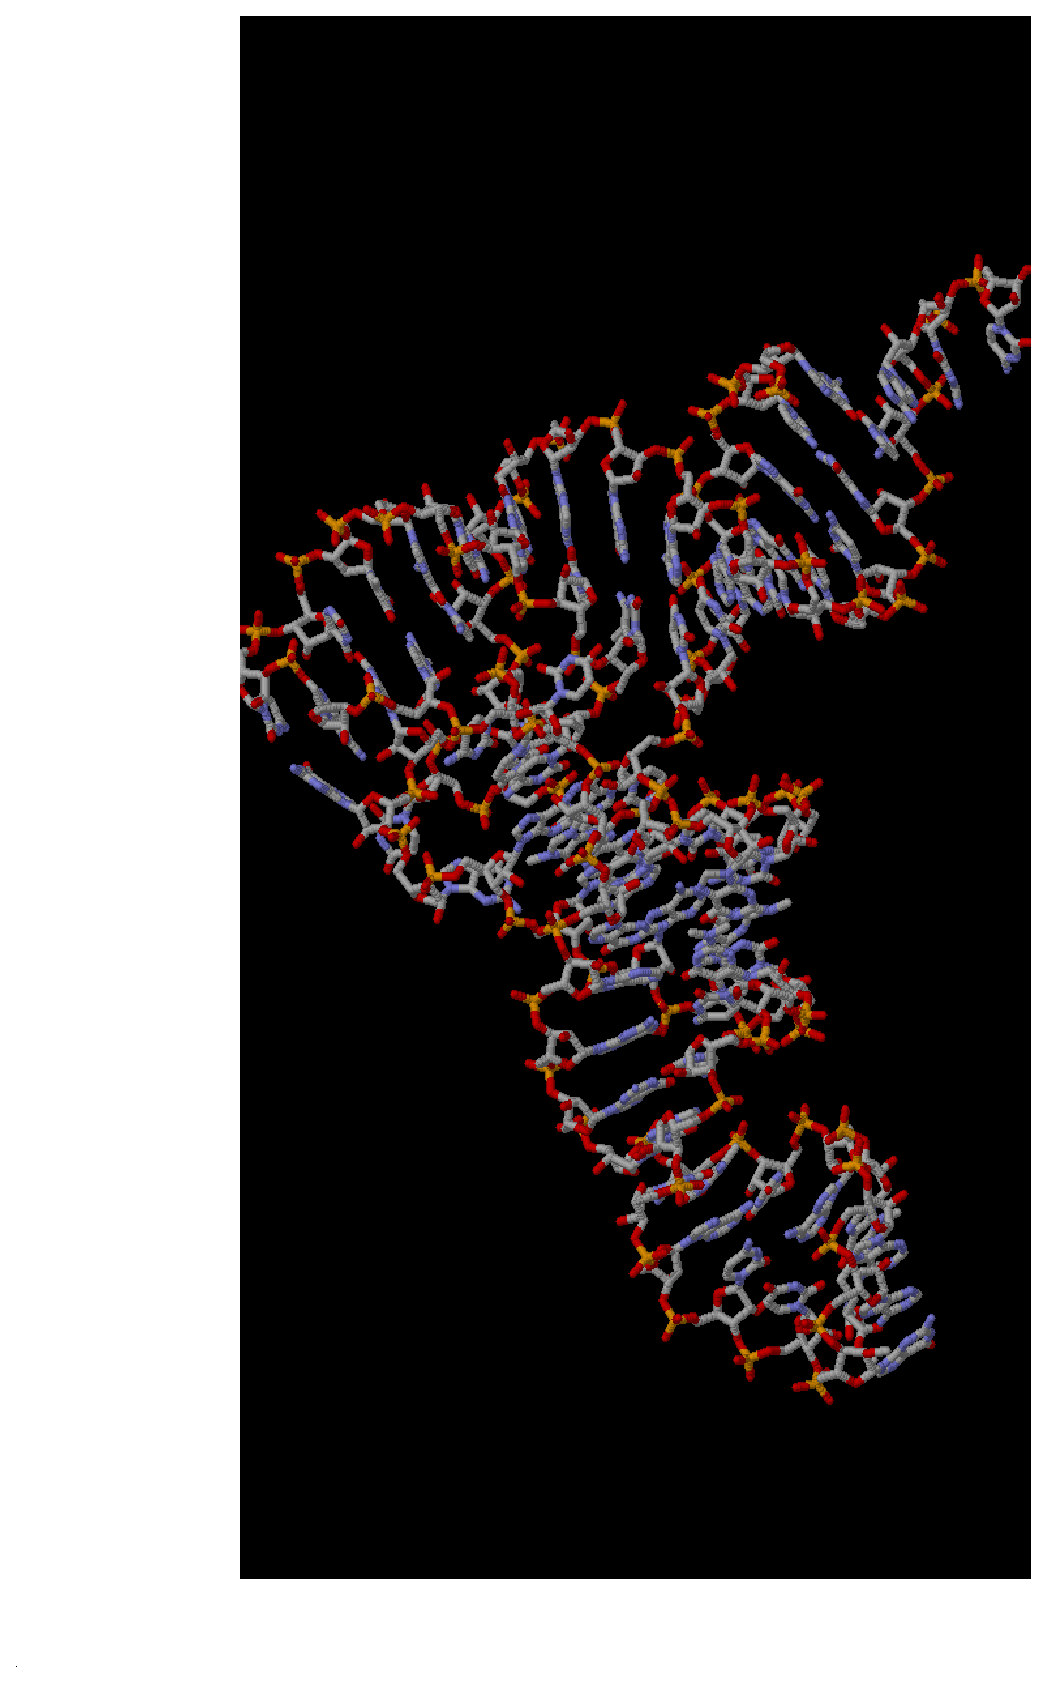
\includegraphics[width=0.8\textwidth]{rna}
%\caption%[]
%{
%Estructura at\'{o}mica de una estructura terciaria de ARN de alta complejidad, generada con el programa
%\htmladdnormallink{RasMol}{http://rasmol.org/}. 
%}
%\label{fig:rna}
%\end{center}
%\end{figure}

Las combinaciones de diferentes cadenas de prote\'\i{}na y/o \'{a}cidos nucleicos para formar una unidad biol\'{o}gica 
funcional se dan ya al nivel de estructura cuaternaria, como ocurre con la 
\htmladdnormallink{hemoglobina humana}{http://en.wikipedia.org/wiki/Hemoglobin}, que funciona como un tetr\'{a}mero, o 
con muchos factores de transcripci\'{o}n que ejercen su papel regulador como mult\'{i}meros, como se muestra en la figura \ref{fig:1cgp}:

\begin{figure}
\begin{center} 
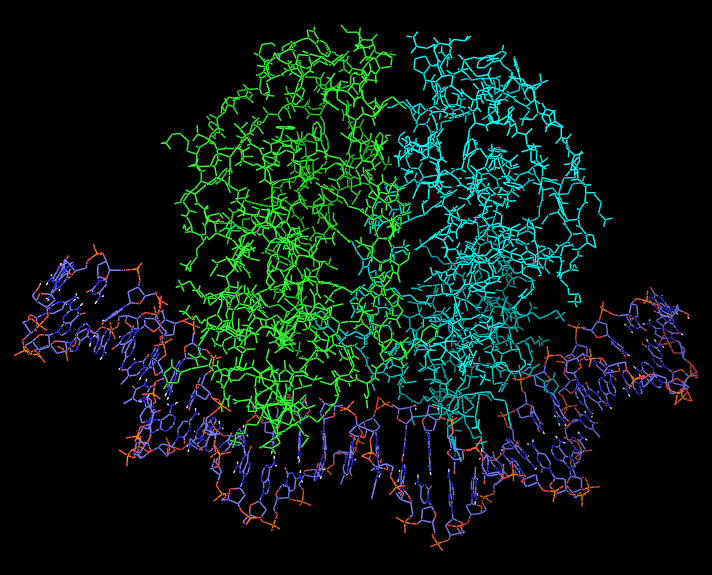
\includegraphics{1cgp_AB}
\caption%[]
{
Estructura del d\'\i{}mero de CRP unido a su ADN operador, generada con el programa
\htmladdnormallink{PyMOL}{http://www.pymol.org} a partir de la entrada \htmladdnormallink{1CGP}{http://www.rcsb.org/pdb/explore.do?structureId=1cgp}
del Protein Data Bank. Las cadenas de prote\'\i{}na est\'{a}n coloreadas en diferentes tonos de verde.
}
\label{fig:1cgp}
\end{center}
\end{figure}

\subsection{Estructura 3D de la cromatina}

La cromatina es una fibra formada por asociaci\'{o}n de DNA gen\'{o}mico y prote\'{i}nas, no s\'{o}lo histonas, y es el constituyente
esencial del n\'{u}cleo celular. Cada vez disponemos de m\'{a}s evidencias de que la estructura de la cromatina es clave para entender 
las funciones de genes, cromosomas e incluso del genoma entero. Algunos de los algoritmos fundamentales que veremos en este curso,
ideados originalmente para el estudio de mol\'{e}culas individuales,
se est\'{a}n reciclando en la actualidad para el estudio de la cromatina, puesto que en cierto modo podemos
modelarla como una fibra lineal; algo parecido a un polip\'{e}ptido al que s\'{o}lo podemos acceder mediante t\'{e}cnicas 
de resoluci\'{o}n limitada. Se puede ampliar este tema en \citet{bau_davide_2014_1066356}.

\begin{figure}
\begin{center} 
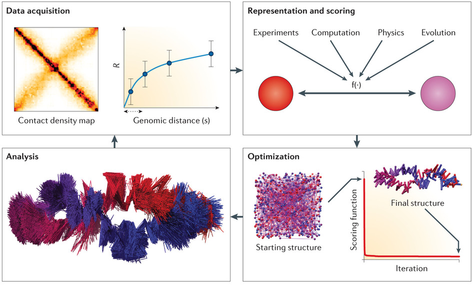
\includegraphics{cromatin}
\caption%[]
{
Diagrama de flujo del proceso de modelado en 3D de la cromatina, tomado de \citep{Dekker2013}. 
Los paneles, comenzando arriba a la izquierda, muestran etapas sucesivas del modelado de un cromosoma bacteriano.
La primera etapa es la captura de datos, que concluye con una matriz de contactos gen\'{o}micos.
la segunda consiste en construir un primer modelo que integre los contactos observados con otros datos disponibles,
por ejemplo evolutivos o f\'{i}sicos. En la tercera etapa se prueban diferentes funciones con el fin de optimizar
el modelo inicial que representa las conformaciones de la cromatina. 
La cuarta etapa es el an\'{a}lisis objetivo del modelo refinado. 
Si los resultados no son satisfactorios es necesario comenzar de nuevo.
Copyright (2013) Springer Nature. 
}
\label{fig:cromatin}
\end{center}
\end{figure}
%https://www.ncbi.nlm.nih.gov/pmc/articles/PMC3874835


\subsection{Relaci\'{o}n entre estructura primaria y terciaria de las prote\'\i{}nas: alineamientos y superposiciones} \label{3dcons}

%En \htmladdnormallink{este}{./papers/chothia_lesk1986.pdf} 
\cite{Chothia1986} analizaron por vez primera la relaci\'{o}n entre la secuencia y la estructura de las prote\'\i{}nas, 
que se puede resumir en esta figura:

\begin{figure}
\htmlimage{scale=1.5}
\begin{center} 
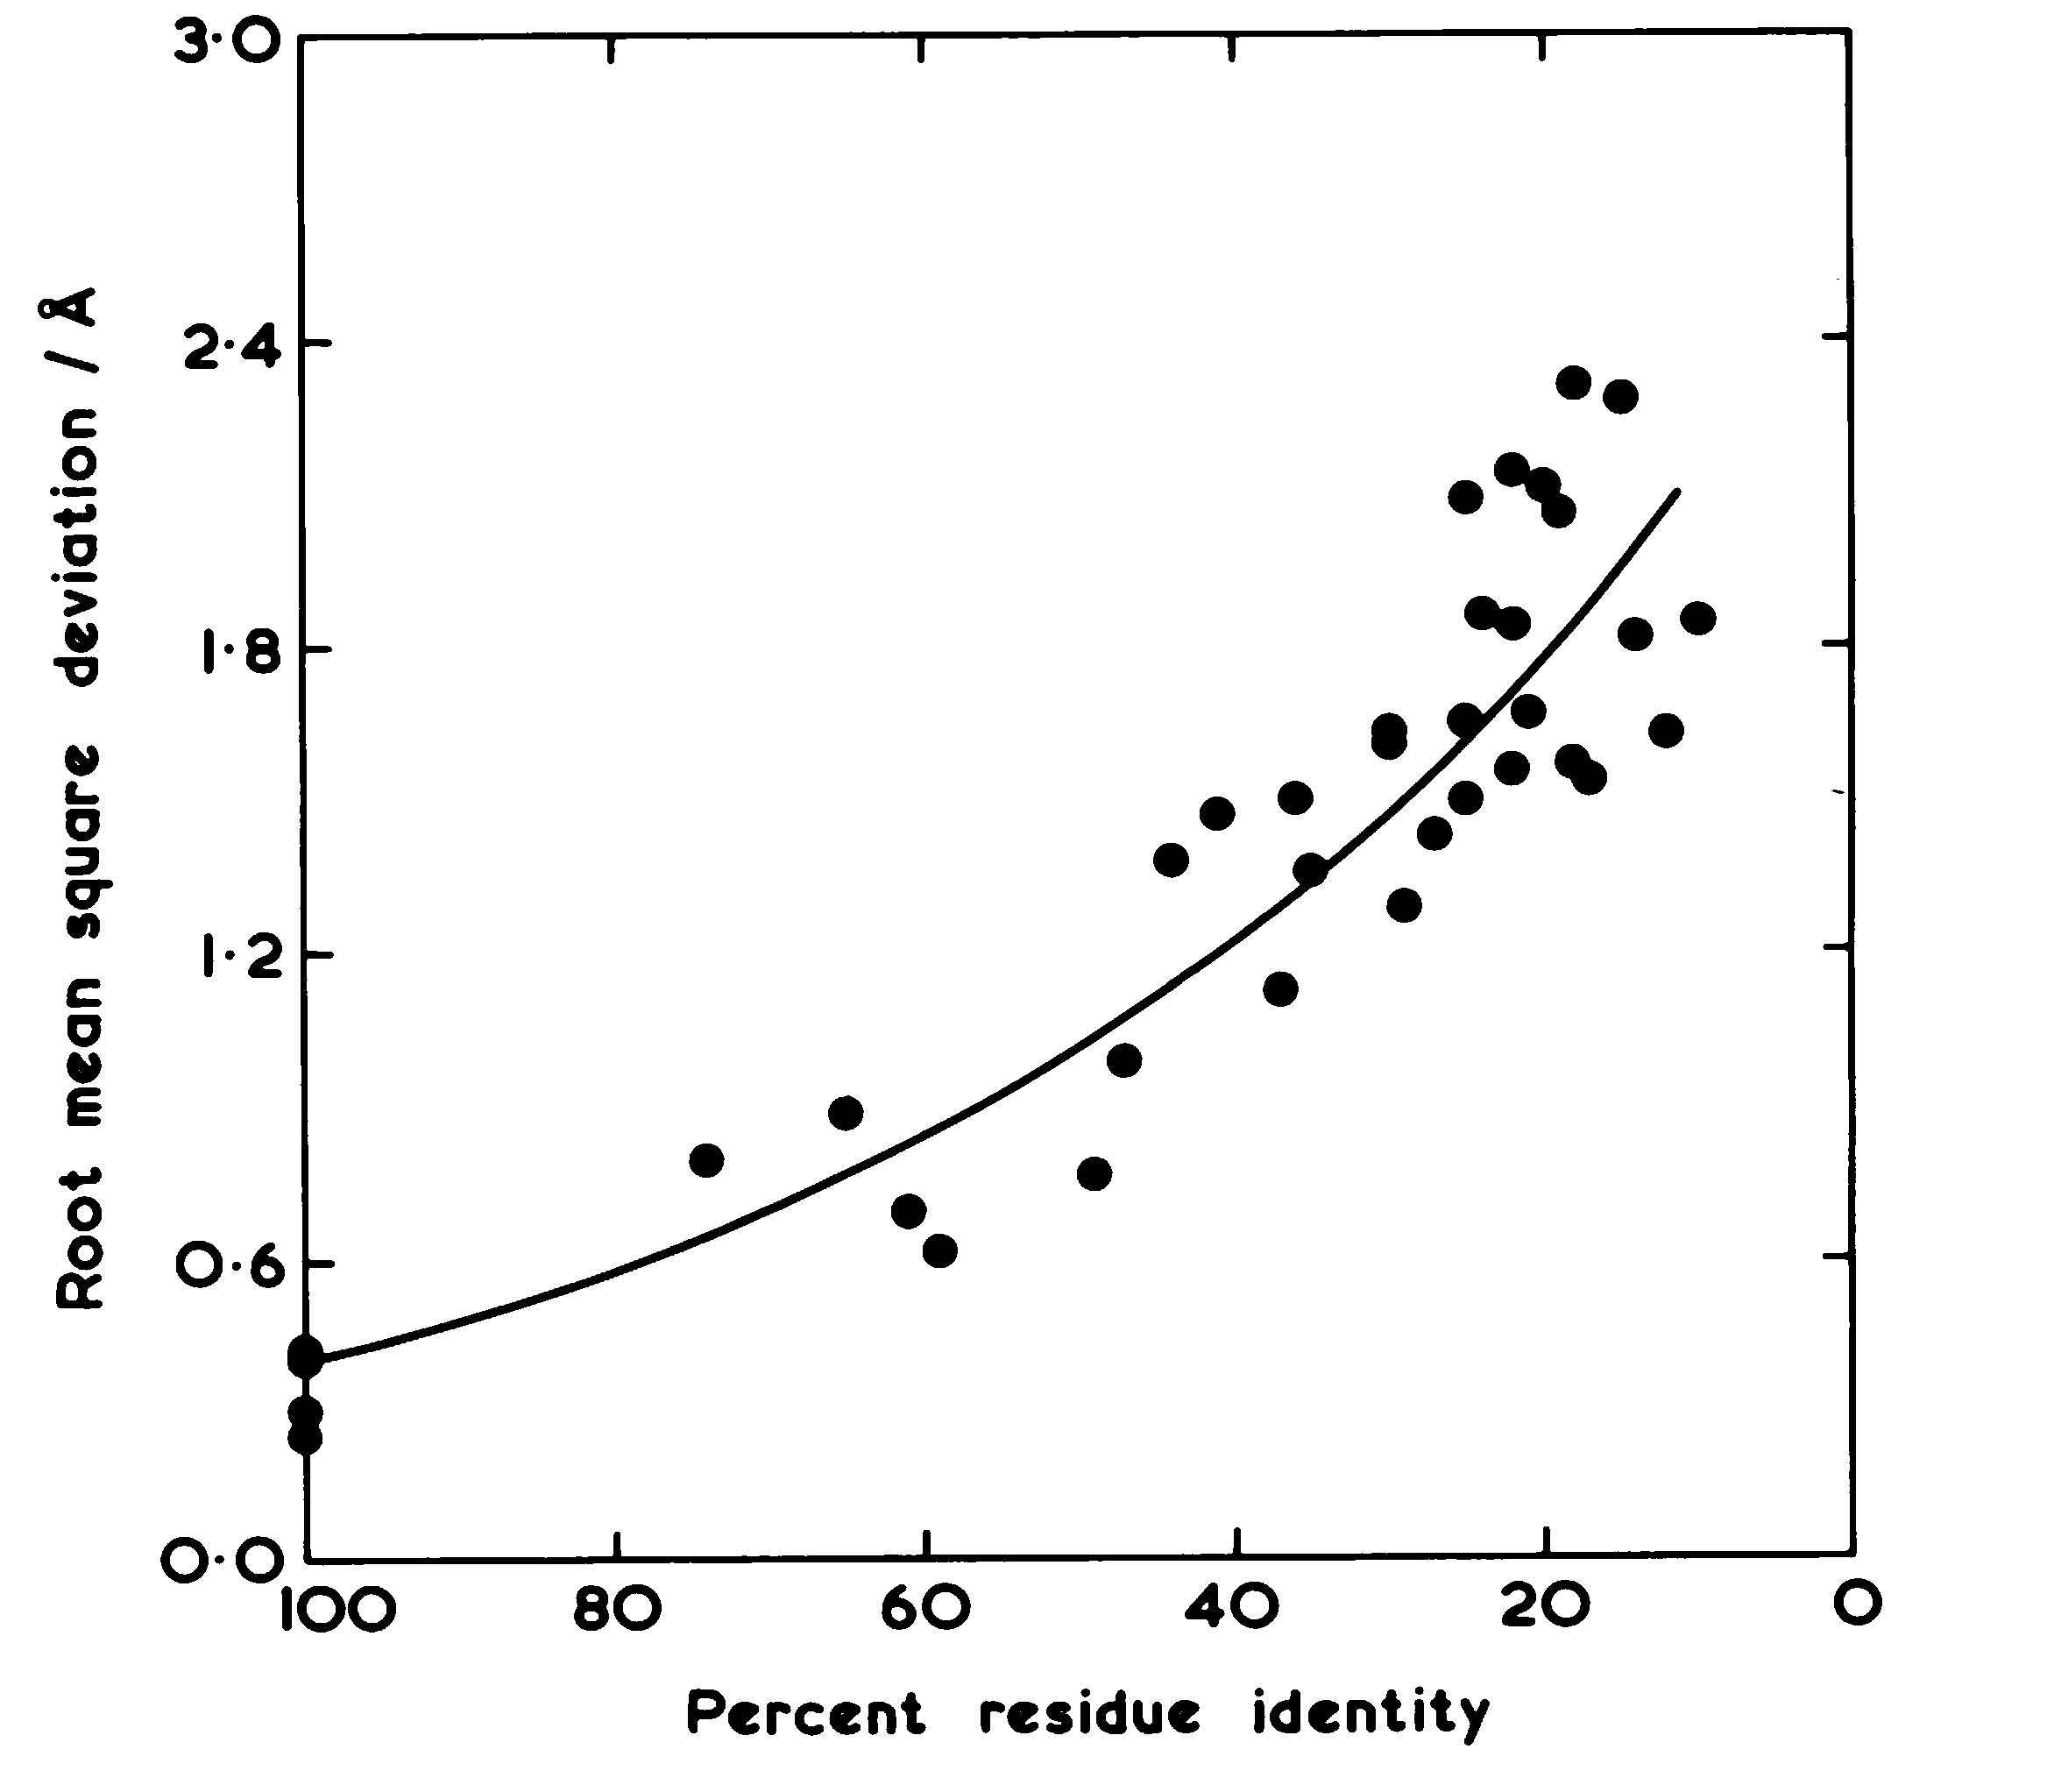
\includegraphics{chothia_lesk}
\caption%[]
{
Correlaci\'{o}n no lineal entre la conservaci\'{o}n de secuencia y estructura de las prote\'\i{}nas,
tomada de \cite{Chothia1986} y reproducida con permiso de los autores.
}
\label{fig:chothia_lesk}
\end{center}
\end{figure}
%https://www.ncbi.nlm.nih.gov/pmc/articles/PMC1166865

Este art\'{i}culo pionero publica la observaci\'{o}n de que a una determinada conservaci\'{o}n entre las secuencias A y B,
calculada por medio de un alineamiento, le corresponde una mayor o menor divergencia en la comparaci\'{o}n de sus estructuras
terciarias, medida en t\'{e}rminos de \htmladdnormallink{desviaciones (RMSD, en Angstrom)}{http://en.wikipedia.org/wiki/Root_mean_square_deviation} 
en las posiciones de sus residuos, dependiendo de si las mutaciones ocurren en el interior (\italics{core}) o exterior del plegamiento. 

\begin{equation}
RMSD = \sqrt \frac{\sum_{i=1}^n dist(C\alpha_{i}^A - C\alpha_{i}^B)^2}{n}
\end{equation} 

Adem\'{a}s, \'{e}ste y otros trabajos posteriores, como \citet{Illergard2009, PascualGarcia2010},
sugieren que la estructura es una propiedad de las prote\'{i}nas que se conserva en mayor medida que la secuencia
durante la historia evolutiva. Lo excepcional es que secuencias similares tengan grandes diferencias estructurales \citep{Kosloff2008}.

\begin{figure}
%\htmlimage{scale=0.5}
\begin{center} 
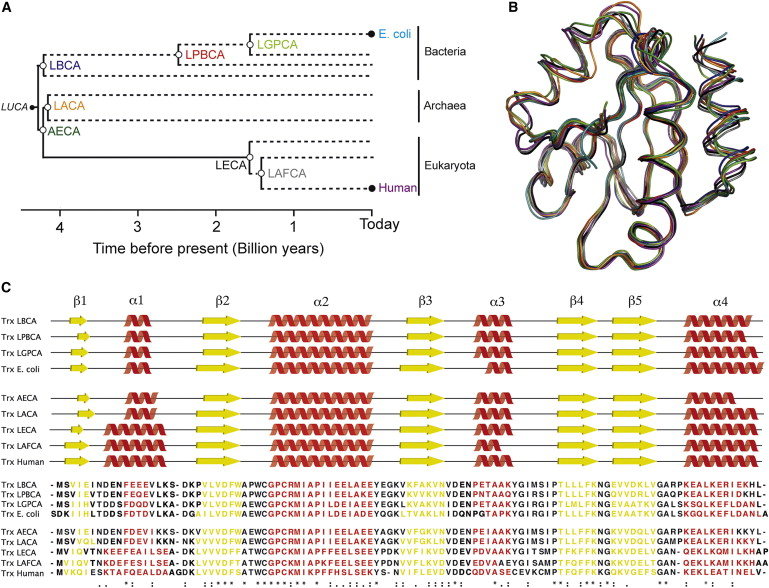
\includegraphics{thioredoxins}
\caption%[]
{
Conservaci\'{o}n de la estructura de tioredoxinas separadas 4 mil millones de a\~{n}os.
(A) \'{A}rbol filogen\'{e}tico moestrando la distancia evolutiva entre H. sapiens y E. coli y algunos de sus ancestros desaparecidos.
(B) Superposici\'{o}n estructural de varias tioredoxinas humanas, de E. coli, y de algunos ancestros prec\'{a}mbricos.
(C) Alineamiento m\'{u}ltiple de las secuencias y estructuras secundarias de las tioredoxinas estudiadas.
Figura reproducida con permiso de \cite{InglesPrieto2013}.
}
\label{fig:thioredoxins}
\end{center}
\end{figure}
%Licensee: 	EEAD-CSIC
%Order Date: 	Jun 5, 2018
%Order Number: 	4362441318100
%Publication: 	Structure
%Title: 	Conservation of Protein Structure over Four Billion Years
%Type of Use: 	reuse in coursepack/classroom materials
%Volveremos a esta observaci\'{o}n muy pronto, pero antes quiero hacer hincapi\'{e}

El panel C de la figura \ref{fig:thioredoxins} es \'{u}til para recordar la correspondencia que se puede establecer 
entre un \textbf{alineamiento} de secuencias y la \textbf{superposici\'{o}n} de las correspondientes estructuras. 
En un alineamiento de secuencia se establece qu\'{e} residuos de una prote\'\i{}na ocupan el mismo lugar en la secuencia
que los de otras prote\'\i{}nas similares. 
En cambio, en una superposici\'{o}n buscamos residuos que ocupan el mismo lugar en la estructura, a los que llamamos  
\textbf{residuos equivalentes}.
Mientras el primero se puede calcular aun sin tener las estructuras, solamente con la secuencia, la superposici\'{o}n
requiere conocer las coordenadas en tres dimensiones de las prote\'\i{}nas en cuesti\'{o}n.
Con aquellas prote\'\i{}nas con estructuras resueltas es posible hacer el siguiente ejercicio,
que tiene como objeto explorar esta correspondencia y aprender que un alineamiento de secuencias con baja identidad
puede contener errores que se hacen patentes al comprobar la correspondiente superposici\'{o}n.


Tomemos por ejemplo las coordenadas de dos 
%\htmladdnormallink{lisozimas}{http://scop.mrc-lmb.cam.ac.uk/scop/data/scop.b.e.c.b.html} del PDB, como
\htmladdnormallink{lisozimas}{http://scop.berkeley.edu/sunid=53955} del PDB, como
\htmladdnormallink{2NWD}{http://www.rcsb.org/pdb/explore/explore.do?structureId=2NWD} y 
\htmladdnormallink{1GD6}{http://www.rcsb.org/pdb/explore/explore.do?structureId=1GD6} 
(\htmladdnormallink{2nwd.pdb}{./files/2nwd.pdb},
\htmladdnormallink{1gd6.pdb}{./files/1gd6.pdb}), 
y alineemos sus secuencias:
\begin{verbatim}
2nwd   KVFERCELARTLKRLGMDGYRGISLANWMCLAKWESGYNTRATNYNAGDRSTDYGIFQIN 60
1gd6   KTFTRCGLVHELRKHGFEEN---LMRNWVCLVEHESSRDTSKTNTNR-NGSKDYGLFQIN 56

2nwd   SRYWCNDGKTPGAVNACHLSCSALLQDNIADAVACAKRVVRDPQGIRAWVAWRNRCQNRD 120
1gd6   DRYWCSKGASPG--KDCNVKCSDLLTDDITKAAKCAKKIYKR-HRFDAWYGWKNHCQG-- 111

2nwd   VRQYVQGCGV 130
1gd6   SLPDISSC-- 119
\end{verbatim}

En este alineamiento las columnas alineadas son parejas de residuos equivalentes o
inserciones/deleciones sin alinear (\textbf{indels}).

Mediante un algoritmo similar al descrito en este %\htmladdnormallink{trabajo}{./papers/McLachlan1979.pdf}
trabajo de \citet{McLachlan1979}, que hace uso de la 
\htmladdnormallink{descomposici\'{o}n en valores singulares}{http://books.google.es/books?id=I2TEgd8-yfsC&lpg=PR1&pg=PA73#v=onepage&q&f=false},
podemos calcular la superposici\'{o}n correspondiente. El siguiente programa, que importa
el m\'{o}dulo \htmladdnormallink{SVD}{./code/SVD.py}, lo implementa:
\verbatiminput{./code/prog3.1.py}

Al cambiar el alineamiento cambia la superposici\'{o}n, demostrando la importancia que tiene la 
variable 'calidad de los alineamientos' si vamos a hacer inferencias estructurales. Sabr\'{i}as editar el c\'{o}digo
para replicar el algoritmo de superposici\'{o}n de \cite{Chothia1986}?



%%%%%%%%%%%%%%%%%%%%%%%%%%%%%%%%%%%%%%%%%%%%%%%%%%%%%%%%%%%%%%%%%%%%%%%%


\section{M\'{e}todos experimentales para el estudio de la estructura y din\'{a}mica de macromol\'{e}culas} \label{metodosExp}

Los principales m\'{e}todos experimentales para determinar la estructura de macromol\'{e}culas son:
\begin{itemize}

%\item Difracci\'{o}n de fibras, usada para el an\'{a}lisis de fibras con patrones repetitivos.

\item Microscop\'\i{}a electr\'{o}nica, para el estudio de grandes complejos moleculares. 
Dentro de esta familia, la microscop\'\i{}a crio-electr\'{o}nica (crio-EM) es la aproximaci\'{o}n m\'{a}s 
prometedora porque ha permitido resolver con alta resoluci\'{o}n grandes complejos moleculares, como ribosomas,
inasequibles por cristalograf\'\i{}a de rayos-X \citep{Callaway2015}.

\item Cristalograf\'\i{}a de rayos-X, aplicable a todas las macromol\'{e}culas, permite obtener 
las descripciones estructurales est\'{a}ticas de m\'{a}s calidad a partir de cristales. 
Un buen libro para leer sobre esto es \cite{Rhodes2000}. 
Las fuentes de radiaci\'{o}n de rayos X de l\'{a}ser de electrones libres (XFEL) permiten estudiar 
cristales peque\~{n}os y prote\'\i{}nas de membrana \citep{Marx2014}.

\item Dispersi\'{o}n de rayos X a bajos \'{a}ngulos (SAXS), que no requiere la obtenci\'{o}n de cristales y 
se ha utilizado para el estudio de prote\'\i{}nas desordenadas.

\item An\'{a}lisis de espectros de resonancia magn\'{e}tica nuclear (NMR), aplicable a todas las 
macromol\'{e}culas, permite estudiar comportamientos din\'{a}micos, como uniones entre mol\'{e}culas y 
movimientos moleculares \citep{Jiang2017}. La construcci\'{o}n de modelos de prote\'\i{}nas a partir de datos de NMR se 
ha logrado automatizar en casos sencillos \citep{Rosato2012,Liu2017}. 
Un libro de referencia sobre esta metodolog\'{i}a es \cite{Cavanagh2000}.

\item An\'{a}lisis de espectros de dicro\'{i}smo circular (CD), 
que permite estimar de manera sencilla en el laboratorio el porcentaje de residuos de una secuencia que adquieren estructura secundaria. 
Los espectros obtenidos se pueden comparar con los de estructuras conocidas \citep{Mavridis2016}. 

\item Espectrometr\'\i{}a de masas de mol\'{e}culas entrecruzadas, 
que ha permitido obtener informaci\'{o}n estructural para modelar complejos de prote\'\i{}nas \citep{Rappsilber2011}. 

\item Captura de conformaciones cromos\'{o}micas, que permiten analizar la organizaci\'{o}n especial de la cromatina celular. Esta 
\htmladdnormallink{familia de m\'{e}todos}{https://en.wikipedia.org/wiki/Chromosome_conformation_capture}
cuantifican las interacciones entre loci cercanos en el espacio pero alejados en la secuencia del cromosoma \citep{bau_davide_2014_1066356}. 

\end{itemize}

Adem\'{a}s de estos m\'{e}todos, enfocados a obtener informaci\'{o}n estructural directamente, hay otras aproximaciones 
basadas en la biolog\'{i}a molecular que permiten extraer informaci\'{o}n estructural indirectamente.
Por ejemplo, la ultrasecuenciaci\'{o}n se usa para dise\~{n}ar prote\'\i{}nas y estudiar mutantes \citep{Wrenbeck2017,Rocklin2017,Butterfield2017}.
Tambien se han empleado ensayos en paralelo para el descubrimiento de regiones desordenadas transactivadoras \citep{Ravarani2018}.

En cualquier caso, los m\'{e}todos experimentales de obtenci\'{o}n de estructuras de macromol\'{e}culas producen 
descripciones at\'{o}micas de variada calidad y resoluci\'{o}n que se suelen describir de manera cuantitativa 
por medio de formatos como el formato \htmladdnormallink{PDB}{http://www.wwpdb.org/documentation/file-format.php}, 
utilizado por el repositorio \htmladdnormallink{Protein Data Bank}{http://www.rcsb.org} (PDB, ver secci\'{o}n \ref{PDBformat}).

En ocasiones puede ser necesario comprobar los datos experimentales crudos sobre los que se construye una estructura del PDB, 
para lo cual podemos recurrir a software como \htmladdnormallink{Coot}{http://en.wikipedia.org/wiki/Coot\_\%28program\%29}. 
Para evaluar independientemente la calidad de una estructura del PDB podemos usar la plataforma 
\htmladdnormallink{MolProbity}{http://molprobity.biochem.duke.edu}.

En el PDB la mayor parte de las estructuras se derivan de cristales o espectros de NMR, y de hecho hay
una buena colecci\'{o}n de prote\'{i}nas que se han resuelto con ambas metodolog\'{i}as, lo que ha permitido concluir 
que son complementarias y que construyen descripciones moleculares muy parecidas, pero no id\'{e}nticas \citep{Brunger1997,Sikic2010,Leman2018}.
De hecho, comparar estructuras resueltas con ambas metodolog\'{i}as permite identificar fragmentos \citep{Hrabe2016} y   
prote\'{i}nas intr\'{i}nsecamente desordenadas \citep{Ota2013}, as\'{i} como prote\'{i}nas que cambian de plegamiento \citep{Porter2018}.

\begin{figure}
\begin{center} 
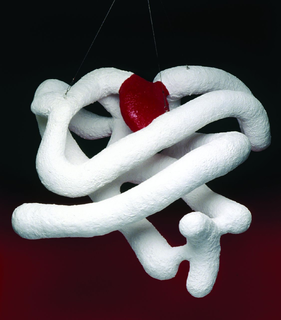
\includegraphics{mioglobina}
\caption%[]
{
Primer modelo en la historia de una prote\'\i{}na, la mioglobina a 6\AA\  de resoluci\'{o}n \citep{Kendrew1958}.
Figura reproducida con permiso de 
\htmladdnormallink{https://www2.mrc-lmb.cam.ac.uk/about-lmb/archive-and-alumni/scientific-models}{https://www2.mrc-lmb.cam.ac.uk/about-lmb/archive-and-alumni/scientific-models}
}
\label{fig:mioglobina}
\end{center}
\end{figure}

\section{El Protein Data Bank y sus formatos} \label{PDBformat}

En las siguientes secciones utilizaremos el formato cl\'{a}sico
\htmladdnormallink{PDB}{http://www.wwpdb.org/documentation/file-format.php} 
(con sus hermanos PDBML y PDBx/mmCIF),
el est\'{a}ndar hist\'{o}rico para codificar la estructura tridimensional de macromol\'{e}culas biol\'{o}gicas, 
sobre todo prote\'\i{}nas y \'{a}cidos nucleicos, por medio de las coordenadas cartesianas de sus \'{a}tomos.
El fichero 
\htmladdnormallink{1LFU}{./files/1lfu.html} muestra el contenido de uno de estos archivos.

Estos archivos pueden visualizarse de forma interactiva usando programas como 
\htmladdnormallink{RasMol}{http://rasmol.org},
\htmladdnormallink{Jmol}{http://jmol.sourceforge.net},
\htmladdnormallink{PyMOL}{http://www.pymol.org},
\htmladdnormallink{Chimera}{https://www.cgl.ucsf.edu/chimera},
o interfaces web como 
\htmladdnormallink{AQUARIA}{http://aquaria.ws}.

Desde 2022 el Protein Data Bank adopt\'{o} por defecto el formato 
\htmladdnormallink{PDBx/mmCIF}{https://mmcif.wwpdb.org} porque supera al PDB a la hora de 
representar estructuras cuaternarias complejas con muchas cadenas. 
El software
\htmladdnormallink{gemmi}{https://github.com/project-gemmi/gemmi} permite convertir entre 
estos formatos.

Hasta 2022 las estructuras del PDB se han nombrado con una combinaci\'{o}n de 4 caracteres, 
empezando por un n\'{u}mero, pero el espacio de nombres posibles se agotar\'{a} pronto y se plantea
que las nuevas estructuras tengan nombres con la estructura \verb+pdb_00017fgz+.

Finalmente, 
aunque en este curso usaremos coordenadas cartesianas, conviene recordar que en muchas aplicaciones
se prefiere usar \htmladdnormallink{coordenadas internas}{http://es.wikipedia.org/wiki/Matriz_Z} 
para hacer operaciones geom\'{e}tricas con mol\'{e}culas de manera eficiente.
